\chapter{Fundamentação teórica}
\label{c.fundamentacao_teorica}

Este capítulo apresenta os fundamentos teóricos que embasam o desenvolvimento deste trabalho. Para compreender o funcionamento e as diferenças entre os algoritmos de compressão de dados abordados, é necessário introduzir alguns conceitos essenciais.

Primeiramente, será apresentada a teoria da informação, a qual fornece o embasamento matemático para a compressão de dados sem perdas, por meio de conceitos como entropia e redundância. Em seguida, serão discutidos os princípios gerais da compressão de dados, com foco nas técnicas sem perdas, suas aplicações e métricas de desempenho. Por fim, serão detalhados os algoritmos clássicos de compressão sem perdas utilizados neste trabalho: Huffman, LZ77, LZW e GZIP, incluindo suas características, funcionamento e aplicações práticas.

A estrutura deste capítulo está organizada da seguinte forma:

\begin{itemize}
    \item \textbf{Seção 2.1} -- Apresenta os principais conceitos da Teoria da Informação, com ênfase na entropia de Shannon e seu papel na compressão de dados;
    \item \textbf{Seção 2.2} -- Discute os fundamentos da compressão de dados sem perdas, destacando seus objetivos, métricas e distinções em relação à compressão com perdas;
    \item \textbf{Seção 2.3} -- Descreve detalhadamente os algoritmos Huffman, LZ77, LZW e GZIP, explicando seus princípios de funcionamento, vantagens, limitações e casos de uso.
\end{itemize}

\section{Teoria da Informação}
\label{sec:teoria-da-informacao}
A Teoria da Informação, proposta por Claude Shannon em 1948, constitui o alicerce teórico para diversos processos de codificação e compressão de dados na ciência da computação e engenharia de comunicações. Seu objetivo central é quantificar a informação contida em uma mensagem e estabelecer limites teóricos para a eficiência da transmissão e armazenamento de dados~\cite{shannon1948}.

\subsection{Quantificação da Informação de Hartley}
Em 1928, Ralph V. L. Hartley publicou o artigo \textit{Transmission of Information}~\cite{hartley1928}, no qual propôs uma medida quantitativa para a informação baseada unicamente em aspectos físicos e objetivos do processo de comunicação. Sua motivação era eliminar fatores subjetivos, como interpretação ou significado, e estabelecer uma definição útil para aplicações em engenharia.

Hartley introduz seu raciocínio a partir da observação de sistemas de comunicação reais, como o sistema de cabo telegráfico submarino operado manualmente. Nesse sistema, o operador utiliza uma chave com três posições, por exemplo, tensão positiva, tensão nula e tensão negativa, cada uma representando um símbolo físico distinto. A mensagem enviada é uma sequência dessas seleções, e o receptor interpreta os sinais registrados por um oscilógrafo em uma fita fotosensível.

O ponto fundamental é que, em cada instante de envio, o operador faz uma escolha consciente entre múltiplos símbolos possíveis. À medida que as seleções ocorrem, mais possibilidades de mensagens são descartadas, o que equivale a dizer que a informação vai se tornando mais específica.

Hartley argumenta que a quantidade de informação transmitida deve depender do número de símbolos disponíveis a cada escolha e do número total de escolhas feitas. Por exemplo, se há \( s = 3 \) símbolos possíveis por escolha e \( n \) escolhas são feitas, o número total de sequências distintas possíveis é:

\[
N = s^n
\]

Esse valor representa a quantidade de mensagens distintas que o sistema é capaz de transmitir fisicamente. No entanto, usar diretamente esse número como medida de informação não é prático, pois ele cresce exponencialmente com o número de seleções. Para obter uma medida linear e proporcional ao número de escolhas, Hartley propõe tomar o logaritmo desse valor:

\[
H = \log_b N = \log_b (s^n) = n \log_b s
\]

Essa expressão garante que:
\begin{itemize}
    \item A medida de informação seja proporcional ao número de escolhas \( n \);
    \item Duas mensagens independentes tenham informação total igual à soma das informações individuais (propriedade de aditividade);
    \item O valor seja expresso em uma unidade prática — como bits, ao usar base \( b = 2 \).
\end{itemize}

\subsubsection*{Exemplos:}

\begin{itemize}
\item \textbf{Exemplo 0:} Considere um sistema em que cada seleção permite escolher entre três símbolos distintos (por exemplo, \( s = 3 \)). Se forem feitas 5 seleções (\( n = 5 \)), o número total de mensagens possíveis é:

	\[
	N = 3^5 = 243
	\]

	A quantidade de informação total transmitida será:

	\[
	H = \log_2 243 \approx 7{,}925 \text{ bits}
	\]

	Ou, usando a fórmula direta:

	\[
	H = 5 \log_2 3 \approx 5 \times 1{,}585 \approx 7{,}925 \text{ bits}
	\]

	Isso significa que, em média, cada seleção transmite aproximadamente 1,585 bits de informação.

    \item \textbf{Exemplo 1:} Suponha um sistema onde o transmissor pode escolher entre 2 símbolos diferentes (como 0 e 1, em um código binário). Uma única escolha transmite:
    \[
    I = \log_2 2 = 1 \text{ bit}
    \]
    Com 8 escolhas, tem-se:
    \[
    H = 8 \log_2 2 = 8 \text{ bits}
    \]

    \item \textbf{Exemplo 2:} Considere agora um sistema com 4 símbolos distintos (por exemplo, A, B, C, D). Cada escolha transmite:
    \[
    I = \log_2 4 = 2 \text{ bits}
    \]
    Após 5 seleções, a quantidade total de informação transmitida é:
    \[
    H = 5 \log_2 4 = 10 \text{ bits}
    \]

    \item \textbf{Exemplo 3:} Em um sistema decimal com 10 símbolos (de 0 a 9), uma única seleção transmite:
    \[
    I = \log_2 10 \approx 3{,}32 \text{ bits}
    \]
    Três seleções transmitiriam aproximadamente:
    \[
    H = 3 \log_2 10 \approx 9{,}97 \text{ bits}
    \]
\end{itemize}

Esses exemplos ilustram que, quanto maior o número de símbolos possíveis por escolha, maior é o conteúdo de informação por escolha individual. A grande sacada de Hartley foi perceber que a informação é proporcional ao número de seleções, e que o logaritmo do número de possibilidades elimina a explosão exponencial, fornecendo uma medida prática e linear.

\subsection{Conteúdo informacional de Shannon}

A abordagem de Hartley, no entanto, assume que todos os símbolos têm igual probabilidade de ocorrência, o que nem sempre é verdadeiro na prática. Para resolver essa limitação, Shannon generalizou o conceito e definiu o conteúdo informacional\footnote{Em inglês, information content, surprisal ou self-information} associada a um evento \( x \) com probabilidade \( P(x) \):

\[
I(x) = -\log_b P(x)
\]

A ideia principal é que o valor informacional de uma mensagem depende do grau em que a mesma é surpreendente. Se um evento altamente provável ocorrer, a mensagem carrega pouca informação; por outro lado, se um evento improvável acontece, diz-se que carrega muita informação. 

Por definição, se \(P(x) = 0\) então \(I(x) = 0\), ou seja, se o evento for impossível, o valor informacional é nulo.

Considere dois eventos distintos:

\begin{itemize}
    \item Evento \( A \): "Vai chover amanhã", com probabilidade \( P(A) = 0{,}9 \);
    \item Evento \( B \): "Vai nevar amanhã", com probabilidade \( P(B) = 0{,}01 \). 
\end{itemize}

Aplicando a fórmula do conteúdo informacional com base 2:

\[
I(A) = -\log_2(0{,}9) \approx 0{,}152 \text{ bits}
\]
\[
I(B) = -\log_2(0{,}01) \approx 6{,}644 \text{ bits}
\]

Isso significa que a ocorrência de \( A \) transmite pouca informação, pois é esperada. Já a ocorrência de \( B \) transmite uma quantidade significativamente maior de informação, pois representa um evento altamente improvável — portanto, mais surpreendente.

Esse exemplo mostra que a informação está relacionada com a incerteza: quanto menor a probabilidade de um evento, maior o seu conteúdo informacional.


\subsection{Entropia}

A entropia de uma fonte, então, é o valor esperado do conteúdo de informação de seus símbolos:

\[
H(X) = - \sum_{i=1}^{n} P(x_i) \log_b P(x_i)
\]

Essa formulação considera a estrutura estatística dos dados, permitindo medir a incerteza média da fonte — e, consequentemente, o limite teórico mínimo para compressão sem perdas.

Considere uma variável aleatória \( X \) que representa o lançamento de uma moeda, onde os possíveis resultados são:

\begin{itemize}
    \item \( x_1 = \text{cara} \), com probabilidade \( P(x_1) = p \)
    \item \( x_2 = \text{coroa} \), com probabilidade \( P(x_2) = 1 - p \)
\end{itemize}

A entropia da variável \( X \) é:

\[
H(X) = -p \log_2 p - (1 - p) \log_2 (1 - p)
\]

Essa função atinge seu valor máximo quando \( p = 0{,}5 \), ou seja, quando a moeda é justa e os dois eventos são igualmente prováveis. Nesse caso:

\[
H(X) = -0{,}5 \log_2 0{,}5 - 0{,}5 \log_2 0{,}5 = -2 \times 0{,}5 \times (-1) = 1 \text{ bit}
\]

Esse valor representa o máximo de incerteza possível para uma variável binária: não se sabe nada sobre qual será o resultado. Por outro lado, se a moeda estiver viciada e sempre cair do mesmo lado (por exemplo, \( p = 0 \) ou \( p = 1 \)), então:

\[
H(X) = -1 \cdot \log_2 1 = 0 \text{ bits}
\]

Ou seja, não há incerteza — o resultado é completamente previsível, e, portanto, não há informação nova sendo transmitida.

\begin{figure}[htbp]
    \caption{\small Entropia de uma moeda em função de \(p\)}
    \centering
    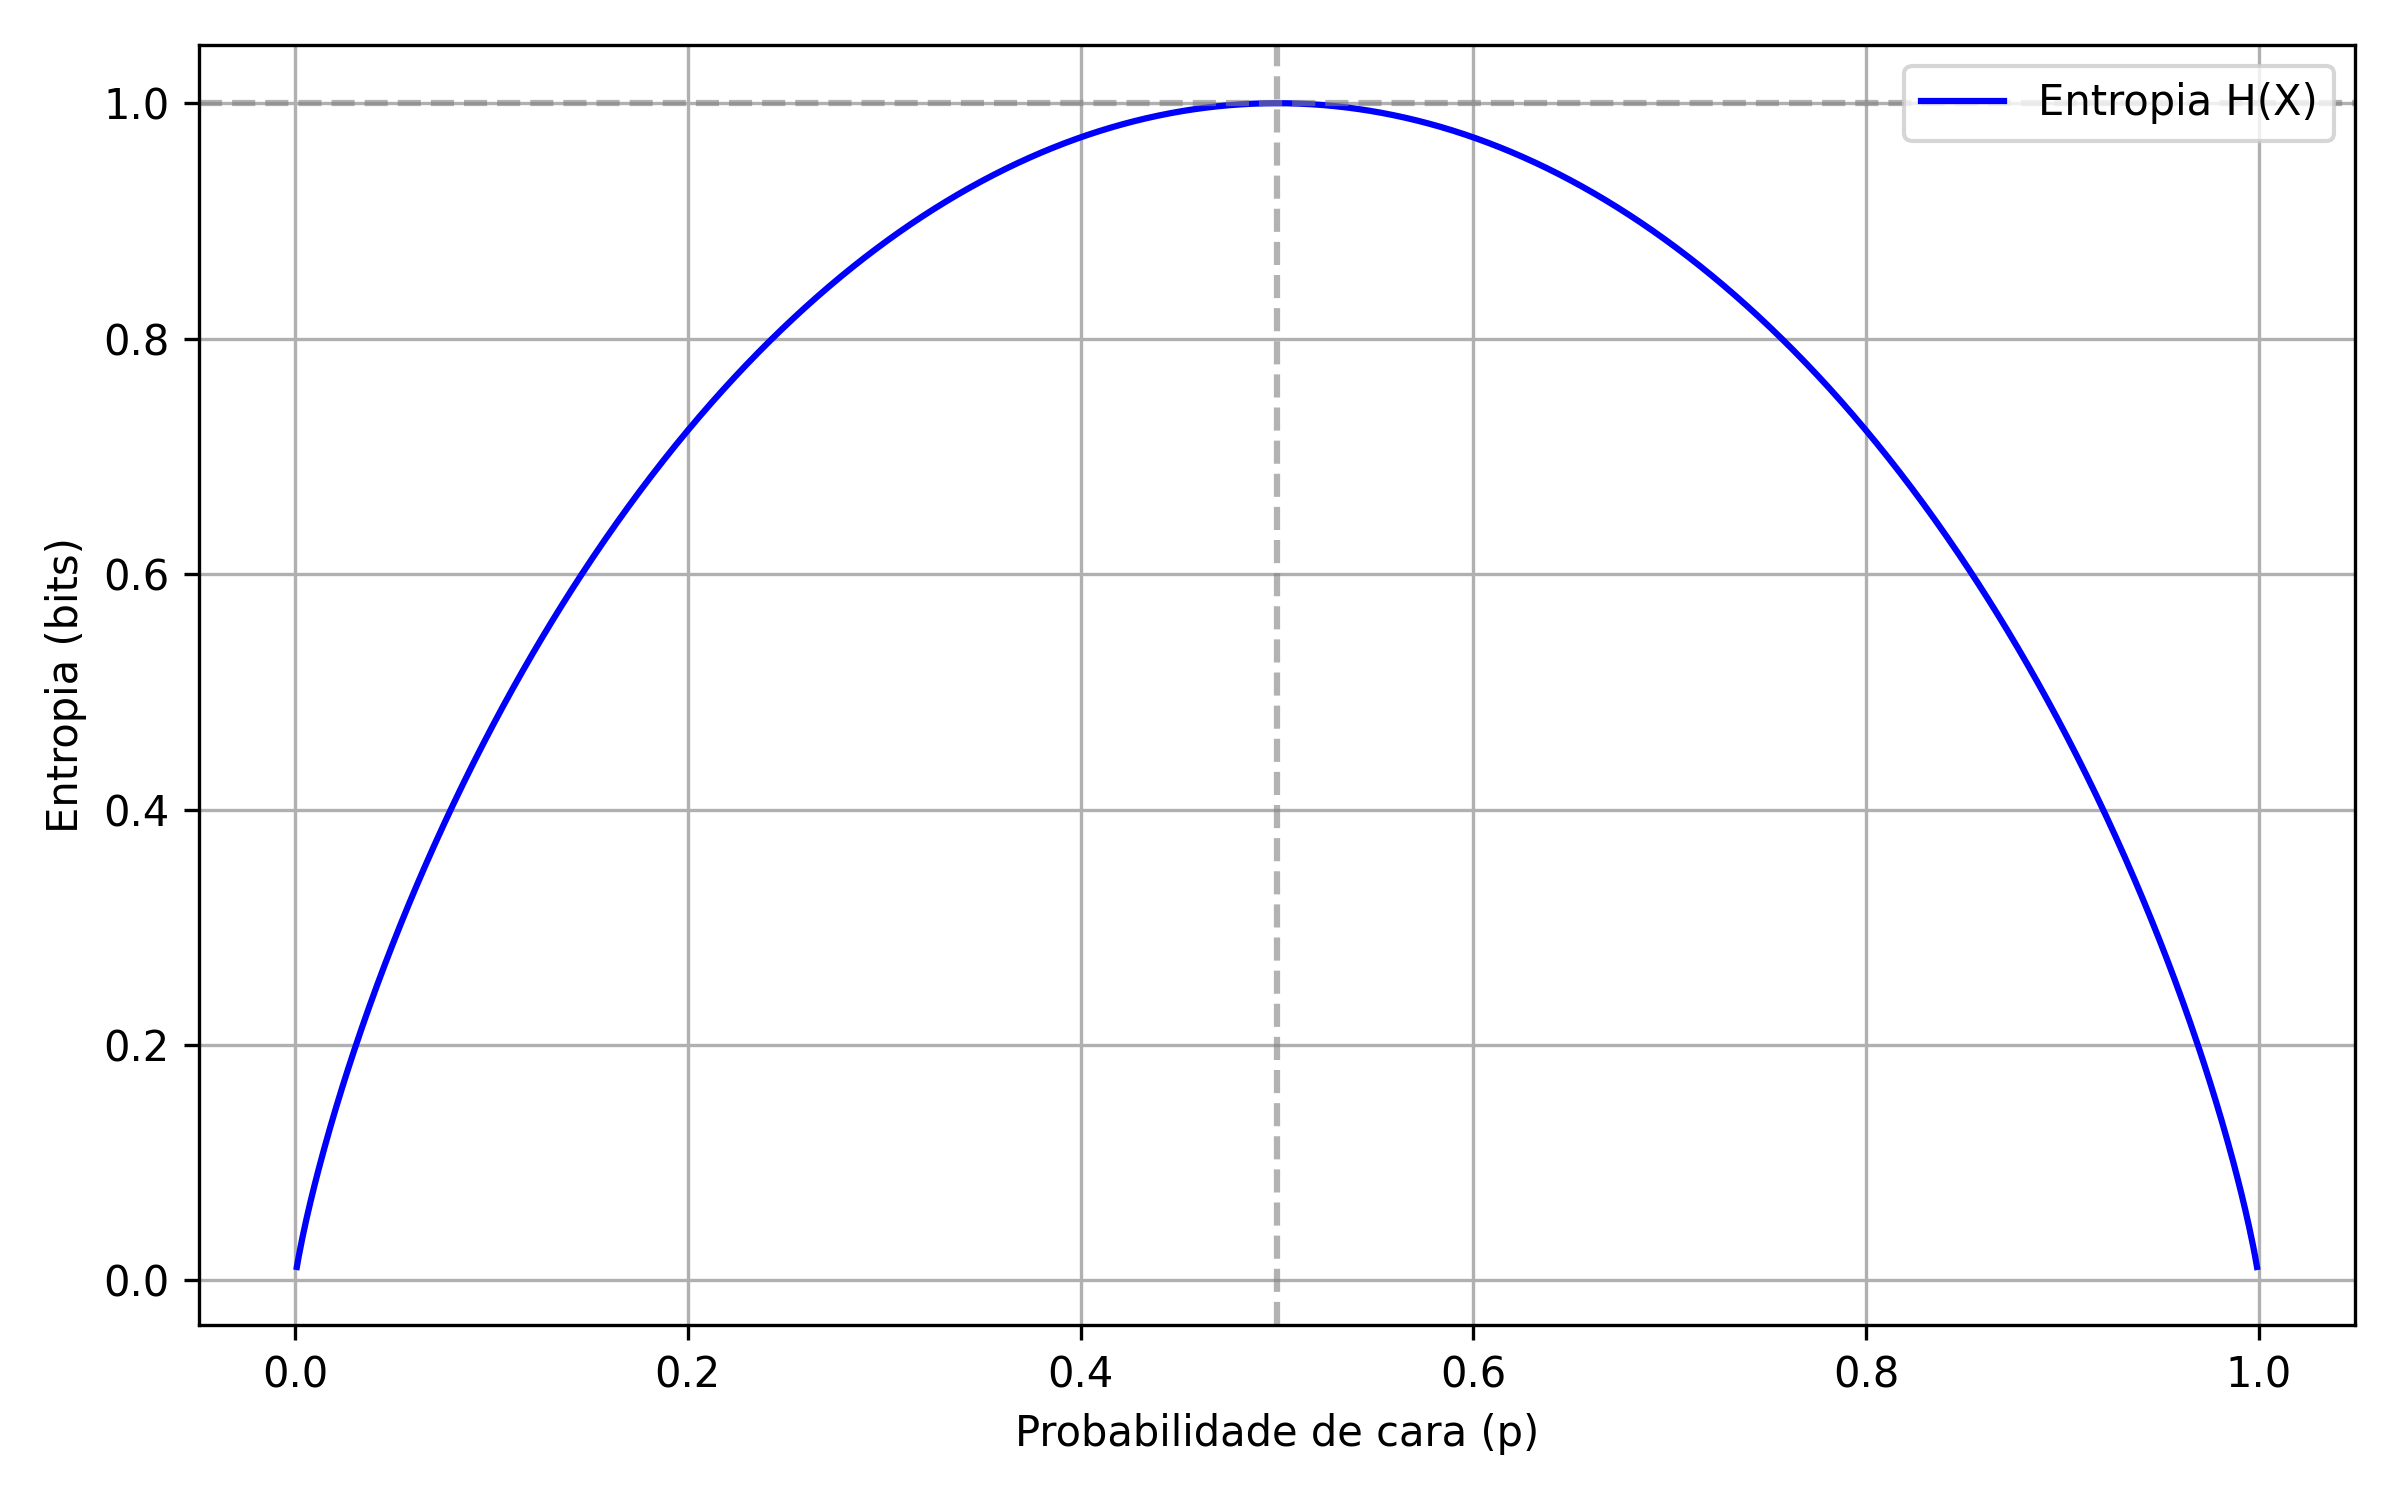
\includegraphics[width=0.8\textwidth]{figs/entropia-moeda.png}
    \label{fig:entropia-moeda}
    \legend{\small Fonte: Elaborada pelo autor}
\end{figure}

\newpage
\subsection{Redundância}

A redundância representa a diferença entre o comprimento médio real de codificação e a entropia da fonte. Em outras palavras, trata-se da quantidade de informação excedente que pode estar presente nos dados, muitas vezes introduzida por razões como segurança, integridade ou simplicidade de codificação. Quanto maior for essa redundância estatística, maior será o potencial de compressão sem perdas.

A relação entre a entropia \( H(X) \) de uma fonte e o comprimento médio \( L \) de um código pode ser expressa por:

\[
R = L - H(X)
\]

onde \( R \) é a redundância. Um código é considerado eficiente quando sua média de bits por símbolo se aproxima da entropia da fonte, ou seja, quando \( R \to 0 \).

O principal objetivo dos algoritmos de compressão de dados é justamente reduzir essa redundância presente na representação original da informação. Ao identificar e eliminar padrões repetitivos, estruturas previsíveis ou codificações desnecessárias, é possível representar os dados com uma quantidade menor de bits, mantendo integralmente a informação. Assim, a compressão atua aproximando o código do limite teórico mínimo imposto pela entropia.

Considere uma fonte com três símbolos e as seguintes frequências:

\begin{center}
\begin{tabular}{ccc}
\toprule
Símbolo & Frequência & Probabilidade \\
\midrule
A & 50 & 0{,}5 \\
B & 30 & 0{,}3 \\
C & 20 & 0{,}2 \\
\bottomrule
\end{tabular}
\end{center}

A entropia dessa fonte, em bits por símbolo, é:

\[
H(X) = - (0{,}5 \log_2 0{,}5 + 0{,}3 \log_2 0{,}3 + 0{,}2 \log_2 0{,}2) \approx 1{,}485 \text{ bits/símbolo}
\]

Após aplicar o algoritmo de Huffman, suponha que os símbolos sejam codificados da seguinte forma:
\begin{itemize}
    \item A → 1 bit
    \item B → 2 bits
    \item C → 2 bits
\end{itemize}

O comprimento médio da codificação é:

\[
L = (0{,}5 \times 1) + (0{,}3 \times 2) + (0{,}2 \times 2) = 1{,}5 \text{ bits/símbolo}
\]

Portanto, a redundância é:

\[
R = L - H(X) = 1{,}5 - 1{,}485 = 0{,}015 \text{ bits/símbolo}
\]

Esse pequeno valor de \( R \) indica que o código de Huffman se aproxima do limite teórico de compressão, demonstrando alta eficiência.

É importante distinguir entre entropia por símbolo e por bit. A entropia calculada a partir da distribuição de probabilidades de uma fonte discreta refere-se, por definição, à quantidade média de informação por símbolo. No processo de compressão:

\begin{itemize}
    \item A entropia total da informação permanece constante (nenhuma informação é perdida);
    \item A entropia por símbolo diminui, pois menos bits são usados por símbolo;
    \item A entropia por bit aumenta, indicando que cada bit carrega mais informação útil.
\end{itemize}

Esse comportamento evidencia a eficácia da compressão, que reduz o volume de dados sem comprometer o conteúdo informacional original.

\section{Compressão de dados}

\section{Algoritmos clássicos de compressão sem perdas}

